\documentclass[border=2pt,svgnames,tikz]{standalone}
\usepackage{fontspec}
\setmainfont{Source Serif 4}
\setsansfont{Source Sans 3}
\setmonofont{Source Code Pro}
\usetikzlibrary{matrix, positioning, calc}

\begin{document}
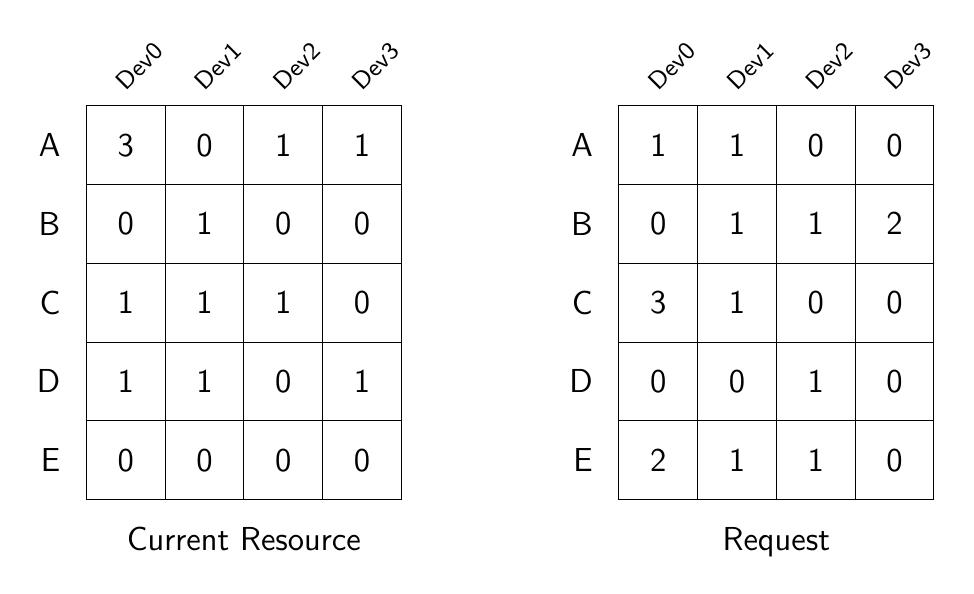
\begin{tikzpicture}[
    cell/.style={draw, minimum size=1.0cm, anchor=center, font=\sffamily\large},
    header/.style={font=\sffamily\small, rotate=45, anchor=south west},
    rowlabel/.style={font=\sffamily\large, anchor=east},
    title/.style={font=\sffamily\large, align=center}
]

% Left Matrix: Current Resource
\matrix (current) [matrix of nodes, nodes={cell}, column sep=-\pgflinewidth, row sep=-\pgflinewidth] {
    3 & 0 & 1 & 1 \\
    0 & 1 & 0 & 0 \\
    1 & 1 & 1 & 0 \\
    1 & 1 & 0 & 1 \\
    0 & 0 & 0 & 0 \\
};

% Row Labels for Left Matrix
\foreach \i/\label in {1/A, 2/B, 3/C, 4/D, 5/E} {
    \node[rowlabel] at ($(current-\i-1.west) + (-0.2, 0)$) {\label};
}

% Column Headers for Left Matrix
\foreach \j/\label in {1/Dev0, 2/Dev1, 3/Dev2, 4/Dev3} {
    \node[header] at (current-1-\j.north) {\label};
}

% Title for Left Matrix
\node[title, below=0.1 of current] {Current Resource};


% Right Matrix: Request
\matrix (request) [matrix of nodes, nodes={cell}, column sep=-\pgflinewidth, row sep=-\pgflinewidth, right=2.5cm of current] {
    1 & 1 & 0 & 0 \\
    0 & 1 & 1 & 2 \\
    3 & 1 & 0 & 0 \\
    0 & 0 & 1 & 0 \\
    2 & 1 & 1 & 0 \\
};

% Row Labels for Right Matrix
\foreach \i/\label in {1/A, 2/B, 3/C, 4/D, 5/E} {
    \node[rowlabel] at ($(request-\i-1.west) + (-0.2, 0)$) {\label};
}

% Column Headers for Right Matrix
\foreach \j/\label in {1/Dev0, 2/Dev1, 3/Dev2, 4/Dev3} {
    \node[header] at (request-1-\j.north) {\label};
}

% Title for Right Matrix
\node[title, below=0.1 of request] {Request};

\end{tikzpicture}
\end{document}
